\documentclass[usepdftitle=false,13pt]{beamer}

\usepackage{beamerthemesplit}

%\usepackage{beamerthemesplit} % need it?
%\usepackage{amsmath} % automatically included by beamer
\usepackage{amssymb} % no longer needed?
\usepackage{amsthm} % no longer needed?
\usepackage{amsfonts} % no longer needed?
\usepackage{graphicx} % automatically included by beamer?
\usepackage{verbatim} % useful for multi-line comments - collision?
%\usepackage{hyperref} % automatically included by beamer
\usepackage{url}

\usepackage{color}


\def\wl{\par \vspace{\baselineskip}}
%\usepackage[usenames,dvipsnames]{xcolor}
\usepackage{beamerthemesplit}
\usepackage{appendixnumberbeamer}



%\usepackage{algorithmic}
% greek support using xetex: compile with xelatex
% (other option: use latex with babel and greektex)
%\usepackage[cm-default]{fontspec} % [cm-default] is needed?
%\usepackage{xunicode}
\usepackage{hyperref}

\usepackage{appendixnumberbeamer}

\setbeamertemplate{bibliography item}[text]

%\usepackage{xltxtra}
%\usepackage{xgreek}
%\newcommand{\el}{\setlanguage{monogreek}}
%\newcommand{\en}{\setlanguage{american}}
%\newcommand{\eng}[1]{\setlanguage{american}#1\setlanguage{monogreek}}
\usepackage[absolute,overlay]{textpos}
\newcommand{\source}[1]{
\begin{textblock*}{4cm}(8.7cm,8.6cm)
    \begin{beamercolorbox}[ht=0.5cm,left,leftskip=2ex]{framesource}
        \usebeamerfont{framesource}\usebeamercolor[fg]{framesource} Source: {#1}
    \end{beamercolorbox}
\end{textblock*}
}

\setbeamercolor{framesource}{fg=gray}
\setbeamerfont{framesource}{size=\tiny}

\addtobeamertemplate{footnote}{\vspace{-6pt}}{\vspace{6pt}}

\renewcommand{\footnoterule}{}

%%%%%%%%%%%%%%%% ΡΥΘΜΙΣΕΙΣ ΜΟΡΦΗΣ %%%%%%%%%%%%%%%%

% font switching works?
%\setromanfont[Mapping=tex-text]{CMU Serif} % also used in math mode
% [Mapping=tex-text] needed for traditional latex combinations
%\setsansfont[Mapping=tex-text]{CMU Sans Serif}
%\setmonofont[Mapping=tex-text]{CMU Typewriter Text} % also used in math mode
%\setmainfont[Mapping=tex-text]{CMU Serif}
% other font choices = FreeSerif etc. or DejaVu Sans etc. or GFS Didot/Elpis/Neohellenic or Kerkis or Calibri or Times New Roman ...
% (use fc-list to find the actual names)

\mode<handout>
{
  % handouts get a slight gray background to make frames noticeable
  \setbeamercolor{background canvas}{bg=black!5}
}


\mode<presentation>% or \mode<beamer>%?
{
  % main theme: specifies colors, fonts, inner and outer (all of these can be overwritten by subsequent commands)
  %\usetheme{Montpellier}
  %\usetheme{Warsaw}
  %\usetheme{Dresden}
  \usetheme{Singapore}

  %\usetheme[numbers,totalnumber,compress,sidebarshades]{PaloAlto}
  %\usetheme{Whale}
  %\usetheme[hideothersubsections,right,width=22mm]{Goettingen}

  % overwrite color theme if needed (there are inner, outer, inner+outer color themes):
  %\usecolortheme{seahorse}
  %\usecolortheme{beaver}
  \usecolortheme{seagull}
  %\usecolortheme{rose}
  % colors can also be specified directly for different parts of the frame:
  %\setbeamercolor{title}{fg=red!80!black,bg=red!20!white}
  %\setbeamertemplate{background canvas}[vertical shading][bottom=white,top=structure.fg!25]
  %\setbeamercolor{normal text}{bg=red!20} % gradient background?
  %\setbeamercolor{background canvas}{bg=} % for transparency

  % overwrite font theme, no actual font differences, just some options for presenting text:
  % invoke with a star to reset the size instead of accumulating
  %\usefonttheme[onlylarge]{structuresmallcapsserif}
  %\usefonttheme[onlylarge]{structurebold}
  %\usefonttheme[onlysmall]{structurebold}
  %\setbeamerfont{title}{shape=\itshape,family=\rmfamily}
  %\setbeamerfont*{frametitle}{size=\normalsize,series=\bfseries}

  % inner and outer themes can also be refined with \useinnertheme{themename} and \useoutertheme{themename}
  %\setbeamersize{text margin left=2em,text margin right=2em}
  %\setbeamersize{sidebar width left=1.5cm}
  %\setbeamersize{someMargin=someWidth} % to change margin sizes

  % other presentation options:
  % this will make invisible stuff not completely invisible:
  %\setbeamercovered{transparent}
  % uncover everything in a step-wise fashion:
  %\beamerdefaultoverlayspecification{<+->}
  % this will supress navigation symbols(?)
  %\setbeamertemplate{navigation symbols}{}
  %\setbeamertemplate{footline}[frame number]
}

  \makeatletter
  \beamer@theme@subsectiontrue 
  \makeatother
% χωρίς διάστημα στην αρχή των παραγράφων (μάλλον δεν χρειάζεται στο beamer)
%\setlength{\parindent}{0pt}
%\setlength{\parskip}{1ex plus 0.5ex minus 0.2ex}

% The table of contents will pop up at the beginning of each section:
\AtBeginSection[] % anything inside the [] will be displayed on section* instead - here nothing
{
  \begin{frame}<beamer>
    \frametitle{}
    \tableofcontents[currentsection]
  \end{frame}
}
% can also be used for subsections:
\begin{comment}
\AtBeginSubsection[] % anything inside the [] will be displayed on section* instead - here nothing
{
  \begin{frame}<beamer>
    \frametitle{}
    \tableofcontents[currentsection,currentsubsection]
  \end{frame}
}
\end{comment}
% other options for toc: pausesections, pausesubsections, currentsubsection, hideothersections, hideothersubsections

% At the start of each part, show an empty slide with the part name:
\AtBeginPart{\frame{\partpage}}


%%%%%%%%%%%%%%%% ΣΤΟΙΧΕΙΑ %%%%%%%%%%%%%%%%

% Τα στοιχεία πρέπει να δηλωθούν πριν αρχίσει το έγγραφο, ώστε να μπουν και στα στοιχεία του PDF

\title[WiFi Networks Research Testbed for Commodity Routers]{WiFi Networks Research Testbed for Commodity Routers}

\author[{Pau, Manos, Eloi}]{Pau, Manos, Eloi}
\institute[{UPC, Guifi.net}]{UPC, Guifi.net}
\date[\today]{\today}
%\date[\today]{\today}

% Δήλωση στοιχείων για το pdf
\hypersetup{
  pdftitle={WiFi Networks Research Testbed for Commodity Routers},
  pdfauthor={Pau, Manos, Eloi},
  pdfsubject={WiFi Testbed},
  pdfkeywords={Networking Testbed, Commodity Routers, wibed}
}


% for authors with multiple affiliations:
%\author[Author, Another]{F.~Author\inst{1} \and S.~Another\inst{2}}
%\institute[Universities of Somewhere and Elsewhere]{
%  \inst{1} Department of Computer Science \\ University of Somewhere \and
%  \inst{2} Department of Theoretical Philosophy \\ University of Elsewhere
%}

% ορισμός logo: με includegraph ics (πακέτο graphics) ή pgfuseimage:
\pgfdeclareimage[height=1.0cm]{project-logo}{pic/wibed-logo}
\logo{\pgfuseimage{project-logo}}
%\logo{\includegraphics[width=1.5cm]{figs/logo}}
%\titlegraphic{\pgfuseimage{university-logo}}
%\titlegraphic{\includegraphics[width=20mm]{upc.png}}




\begin{document}
\title[WiBed\hspace{20em}\insertframenumber/\inserttotalframenumber]{WiFi Networks Research Testbed for Commodity Routers}  
\author[Pau@Guifi,\{Manos,Eloi\}@UPC ]{ Pau, Manos, Eloi\\
 }

\date{\today} 

\frame{\titlepage}

%\section[Outline]{}
%\frame{\tableofcontents}



\section{Introduction}
\subsection{Motivation}

\begin{frame}\frametitle{Wait what?}

\begin{figure}[h!]
\begin{center}

\includegraphics[width=0.45\textwidth]{pic/Wiibed}
\end{center}
\end{figure}

\end{frame}



\begin{frame}\frametitle{Really?}

	\begin{itemize}
		\item Are you into networking?
		\pause
		\item Do you want to do realistic experiments?
		\pause
		\item Are you sick of all the virtualization hype?
		\pause
		\item Are you desperate to perform L2 or lower experiments?
	\end{itemize}
	\pause
	\begin{center}
	Then you need:\\
	
\includegraphics[width=0.35\textwidth]{pic/wibed-logo}
	\end{center}

\end{frame}

\subsection{What is that?}

\begin{frame}\frametitle{What is WiBed?}

	WiBed is:
	\begin{itemize}
		\item A software platform aimed at deploying network experiments
		\item Also an OpenWRT-based platform to easily deploy and manage your mesh network
		\item Designed to run on commodity (cheap) IEEE802.11 routers
		\item Your best option for wireless networking experiments :)
	\end{itemize}

\end{frame}


\begin{frame}\frametitle{What is WiBed?}

	but WiBed is also:
	\begin{itemize}
		\item An effort started by "hackers" in the WBMv6
		\item Complement Community-Lab.net testbed (Low Cost, Low layer Experiments)
		\item Fast-installed self-organized mesh network
	\end{itemize}

\end{frame}

\section{Architecture}
\subsection{Overview}
\begin{frame}\frametitle{Architecture Overview}

\begin{figure}[h!]
\begin{center}
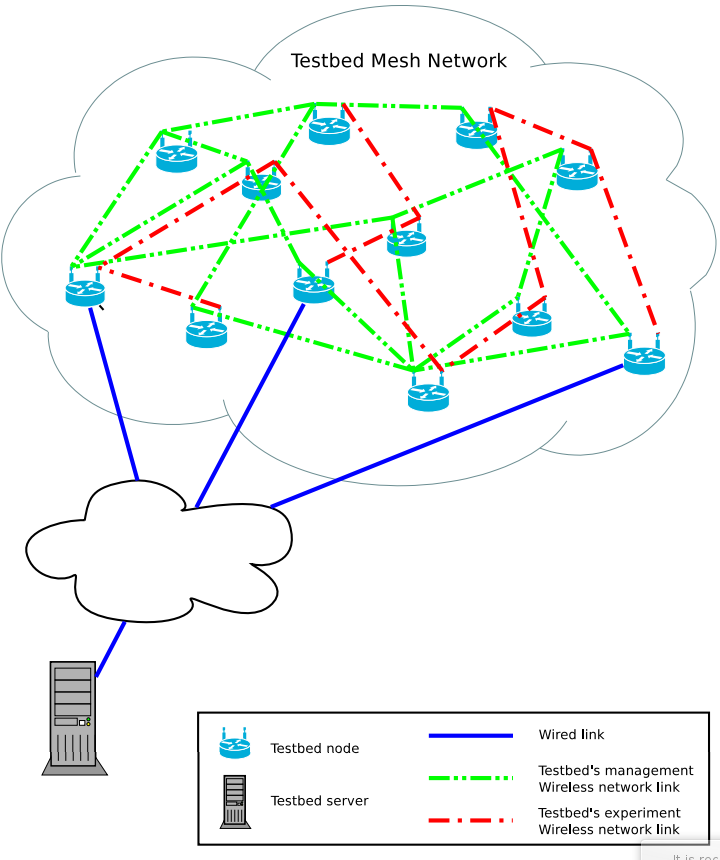
\includegraphics[width=0.45\textwidth]{pic/wibed_arch}
\caption{WiBed Architecture}
\label{fig:wmn}
\end{center}
\end{figure}

\end{frame}

\begin{frame}\frametitle{Design Overview}

	\begin{itemize}
		\item Nodes behave like FSM (idle-prepare-deploy-run-finish-idle)
		\item Communication with server through management mesh network
		\item REST-API pulling mechanism: every N seconds nodes pull state info and orders from server
		\item Node access mainly from the server web-UI
		\item Based on OpenWrt trunk
		\item Organized in packages, OpenWRT-compatible feed
		\item Management Network based on batman-adv 
	\end{itemize}
\end{frame}


\subsection{Implementation}

\begin{frame}\frametitle{Hardware}

	\begin{itemize}
	\item Node must be compatible with OpenWRT Linux (minimum 4MB flash)
	\item Node must have at least two radios (one for mgmt, one for experiments)
	\item Node must have at least one USB port (to store the overlay)
	\end{itemize}

	\begin{figure}[h!]
	\begin{center}
	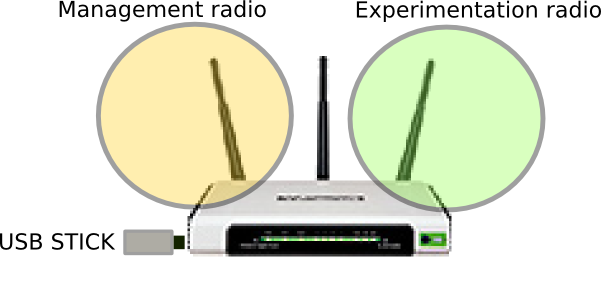
\includegraphics[width=0.6\textwidth]{pic/nodehw}
	  \caption{WiBed Node hardware}
	\label{fig:funct}
	\end{center}
	\end{figure}
\end{frame}

\begin{frame}\frametitle{Diagram}

	\begin{itemize}
	\item Nodes self-configure during the first boot
	\item IP address, hostname, ssid, etc. based on MAC address
	\item Experiments are overlays which are installed in the nodes
	\item Once an experiment finish, the overlay is removed and node goes back to initial state
	\end{itemize}

	\begin{figure}[h!]
	\begin{center}
	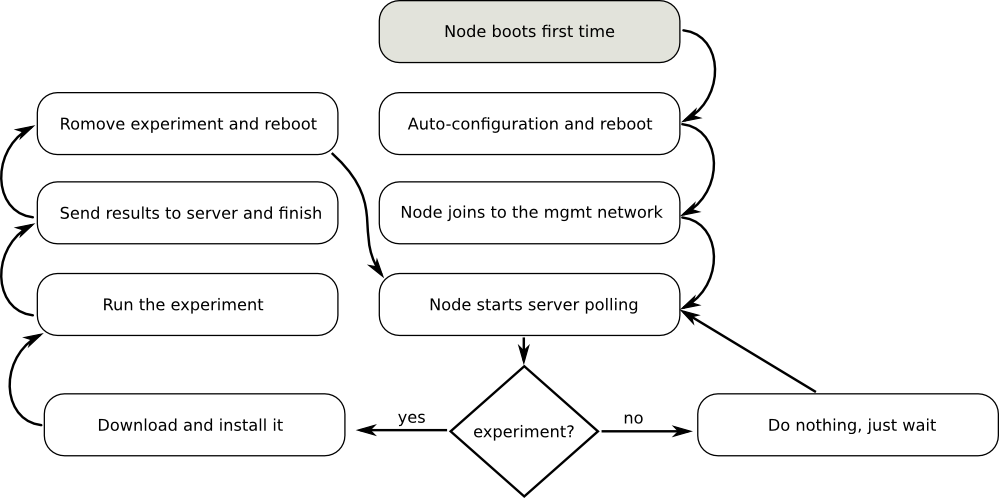
\includegraphics[width=0.6\textwidth]{pic/functdia}
	  \caption{WiBed Node functional diagram}
	\label{fig:funct}
	\end{center}
	\end{figure}
\end{frame}

\begin{frame}\frametitle{OverlayFS 1/2}

\begin{figure}[h!]
\begin{center}
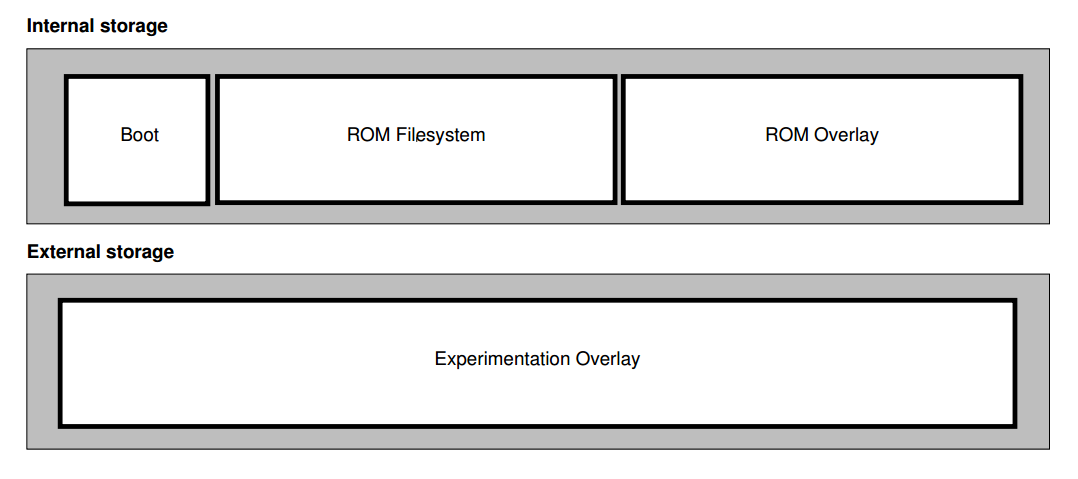
\includegraphics[width=0.6\textwidth]{pic/firmfs1}
\caption{WiBed Node Filesystem}
\label{fig:wmn}
\end{center}
\end{figure}

\end{frame}

\begin{frame}\frametitle{OverlayFS 2/2}


\begin{columns}[c] % the "c" option specifies center vertical alignment
    \column{.5\textwidth} % column designated by a command
		\begin{figure}[h!]
		\begin{center}
		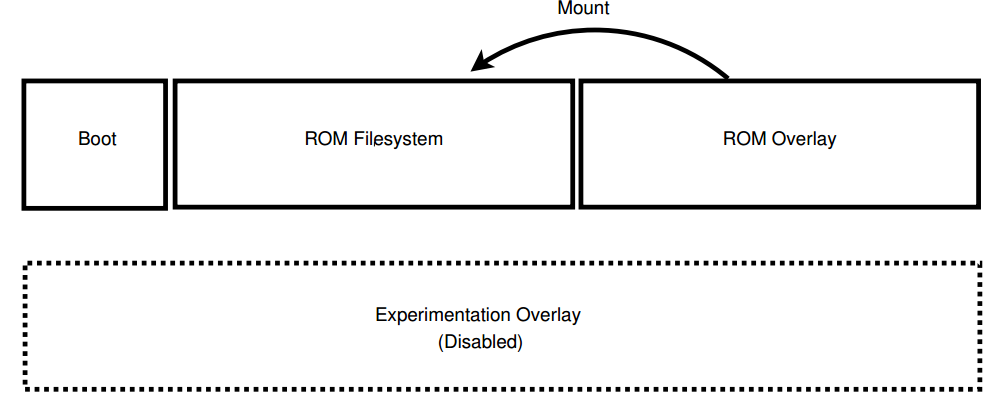
\includegraphics[width=1.0\textwidth]{pic/firmfs2}
		\caption{Node in IDLE state}
		\label{fig:wmn}
		\end{center}
		\end{figure}
   	\column{.5\textwidth}
  		\begin{figure}[h!]
		\begin{center}
		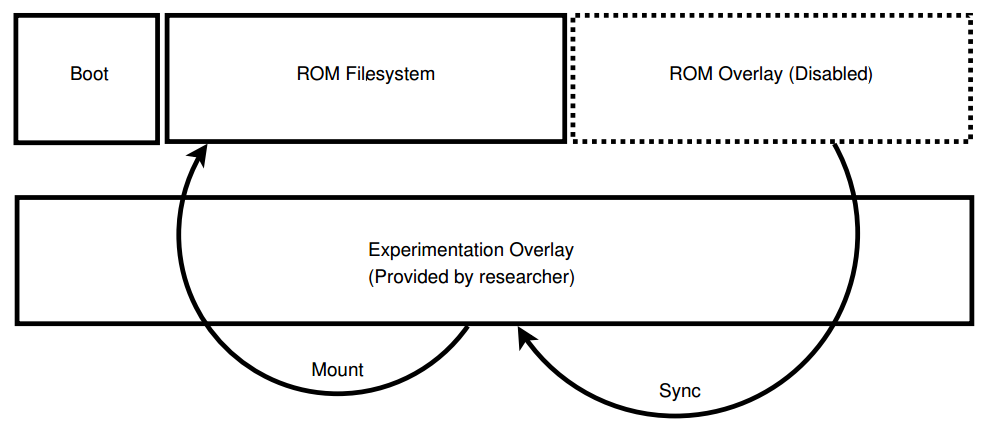
\includegraphics[width=1.0\textwidth]{pic/firmfs3}
		\caption{Node performing experiment}
		\label{fig:wmn}
		\end{center}
		\end{figure}  
   	\end{columns}

\end{frame}






\begin{frame}\frametitle{Config file}

	\begin{itemize}
	\item WiBed uses UCI to manage the configuration
	\item It is flexible and allows many options
	\\
	For instance, management network device can be defined as ``list ifaces radio2/radio1'' meaning if radio2 exists, it will be used, otherwise radio1
	\end{itemize}

	\begin{figure}[h!]
	\begin{center}
	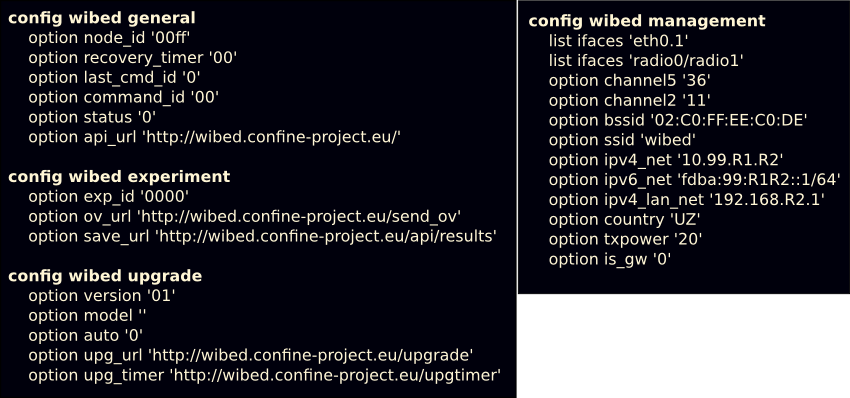
\includegraphics[width=0.6\textwidth]{pic/config}
	  \caption{WiBed Node functional diagram}
	\label{fig:funct}
	\end{center}
	\end{figure}
\end{frame}



\subsection{WiBed Server}



\begin{frame}\frametitle{Wibed Server}
	\begin{itemize}
		\item \textit{Server}:  \texttt{Tornado Web Server}
		\item \textit{Our system}: \texttt{Flask} app + \texttt{SQLite}
		\item A REST API for interaction with nodes
		\item A web interface for interaction with users
	\end{itemize}

\end{frame}

\section{End of story}

\begin{frame}\frametitle{More info}

	\begin{itemize}
		\item {\color{blue} \href{http://wiki.confine-project.eu/wibed:start}{Wiki}}
		\item {\color{blue} \href{http://wiki.confine-project.eu/_media/wibed:wibed-7pages.pdf}{Paper}}
		\item {\color{blue} \href{http://redmine.confine-project.eu/projects/wibed}{Repo}}
		\item Us 
	\end{itemize}

\end{frame}

\begin{frame}\frametitle{Got you!}

	\begin{figure}[h!]
	\begin{center}
	
\includegraphics[width=0.6\textwidth]{pic/nerd}
	\label{fig:sdn}
	\end{center}
	\end{figure}

\end{frame}




\begin{comment}

\begin{frame}\frametitle{Wireless Mesh Networks}

\begin{figure}[h!]
\begin{center}
\includegraphics[width=0.8\textwidth]{figs/wmn}
\caption{Typical WMN architecture.\footnote{\tiny Source: \cite{akyi05}}}
\label{fig:wmn}
\end{center}
\end{figure}

\end{frame}



\begin{frame}\frametitle{Community Network testbed}

%Now Imagine multiple community networks. -> This is community-lab

\begin{figure}[h!]
\begin{center}
\includegraphics[width=0.7\textwidth]{figs/cntestbed}
\caption{A Community Network Testbed. \footnote{\tiny Source: Commmunity-Lab, demo at the IEEE Peer-to-Peer Conference, Sept 3, 2012\\
\url{http://wiki.confine-project.eu/_media/pub:community-lab.pdf}}}
\label{fig:cntestbed}
\end{center}
\end{figure}

\end{frame}



\section{Introduction}

\subsection{Community-Lab}

\begin{frame}\frametitle{Architecture}

\begin{figure}[h!]
\begin{center}
\includegraphics[width=0.9\textwidth]{figs/confarch1}
\caption{Community-Lab architecture.\footnote{\tiny Source: \cite{neum12}}}
\label{fig:confarch}
\end{center}
\end{figure}

\end{frame}


\begin{frame}\frametitle{Abstract Experiment View}

\begin{figure}[h!]
\begin{center}
\includegraphics[width=0.6\textwidth]{figs/confarch}
\caption{Abstract view of Community-Lab architecture.\footnote{\tiny Source: \url{http://wiki.confine-project.eu/arch:start}}}
\label{fig:confarch1}
\end{center}
\end{figure}

\end{frame}

\subsection{Software Defined Networking}

\begin{frame}\frametitle{Overview}


\begin{figure}[h!]
\begin{center}
\includegraphics[width=0.6\textwidth]{figs/sdn}
\caption{Abstract view of SDN.\footnote{\tiny Source: \cite{shen11} }}
\label{fig:sdn}
\end{center}
\end{figure}



\end{frame}


\begin{frame}\frametitle{OpenFlow Idea}

\begin{figure}[h!]
\begin{center}
\includegraphics[width=1.0\textwidth]{figs/of}
\caption{OpenFlow idea. \footnote{\tiny Source: Brand Hedlund's blog\\
\url{http://bradhedlund.com/2011/04/21/data-center-scale-openflow-sdn/}}}
\label{fig:of}
\end{center}
\end{figure}

\end{frame}

\begin{frame}\frametitle{OpenFlow Switch}

\begin{figure}[h!]
\begin{center}
\includegraphics[width=0.5\textwidth]{figs/ofarch}
\caption{Idealized OpenFlow Switch.\footnote{Source: \tiny \cite{mcke08}}}
\label{fig:ofarch}
\end{center}
\end{figure}

\end{frame}


\subsection{Motivation}
\begin{frame}\frametitle{Motivation}

\textbf{Case}:\\
No L2 experiments in Community-Lab.
\wl

\textbf{Goal}:\\
Design and implement a system for a CN testbed that allows L2 experiments and is based on SDN.
\wl

\textbf{Scenario}:\\
Manage the L2 topology of a set of nodes



\end{frame}



\section{Architecture}

\subsection{Challenges }

\begin{frame}\frametitle{Due to...}

\textbf{Wireless Mesh Network Nature} \hyperlink{supplemental1}{\beamerbutton{CNs and WMNs}}\\
\pause
\begin{itemize}
\item \textit{Challenge 1}: Wireless Mesh Network Nature 
\pause
\item \textit{Challenge 2}: Link Capacity
\end{itemize}
\pause
\wl
\textbf{CNs and CN Testbeds}\\
\pause
\begin{itemize}[<+->]
\item \textit{Challenge 3}: Device and Protocol Diversity 
\item \textit{Challenge 4}: Communication with Non-Testbed Nodes 
\item \textit{Challenge 5}: No Out-of-band Channels
\end{itemize}

\end{frame}





\subsection{Decisions}


\begin{frame}[label=main]
\frametitle{Decision Categories}
\begin{itemize}
\item Basic Infrastructure \wl \wl
\item Functionality \wl \wl
\item Optimizations
\end{itemize}
\hyperlink{supplemental}{\beamerbutton{Tackling Challenges}}
\end{frame}



\begin{frame}\frametitle{Basic Infrastructure}

\begin{itemize}[<+->]
\item \textbf{Decision 1}: OF Software Switches on the host side of testbed nodes \wl \wl
\item \textbf{Decision 2}: OF Controller in Testbed Server
\end{itemize}

\end{frame}


\begin{frame}\frametitle{Functionality}

\begin{itemize}[<+->]
\item \textbf{Decision 3}: L2 mesh routing protocol for multihop L2 connectivity \\ \begin{center} \includegraphics[width=0.3\textwidth]{figs/archstack} \end{center}
\item \textbf{Decision 4}: Control plane through management interface, data plane through local interface
\end{itemize}

\end{frame}


\begin{frame}\frametitle{Optimizations}

\begin{itemize}[<+->]
\item \textbf{Decision 5}: Use OF in proactive mode \wl \wl
\item \textbf{Decision 6}: Local Proxy OF controller in testbed nodes
\end{itemize}

\end{frame}


\subsection{Overview}

\begin{frame}\frametitle{Architecture Overview}

\begin{figure}[h!]
\begin{center}
\includegraphics[width=0.8\textwidth]{figs/architecture}
\caption{Overview of the architecture.}
\label{fig:arch}
\end{center}
\end{figure}

\end{frame}



\section{Implementation}

\subsection{Software Developed}

\begin{frame}\frametitle{Poxy}

Poxy implements a proxy for the controller-switch OFP connection, on top of the POX OF controller.
\begin{figure}[h!]
\begin{center}
\includegraphics[width=0.6\textwidth]{figs/Poxy}
\caption{Basic idea of Poxy}
\label{fig:poxy}
\end{center}
\end{figure}

\end{frame}


\begin{frame}\frametitle{Pongo}

Pongo is an attempt to integrate POX with Django in order to administer L2 experiments in a collection of nodes.

\wl
\begin{center}
\includegraphics[width=0.3\textwidth]{figs/pongo0}
\end{center}
\pause

A specific version of Pongo was created to achieve also CONFINE integration.
\begin{center}
\includegraphics[width=0.6\textwidth]{figs/pongo}
\end{center}






\end{frame}

\subsection{External Software}

\begin{frame}\frametitle{External Software}

\begin{itemize}
\item \textbf{CONFINE Software}: CONFINE Node Software System, CONFINE Controller Software
\item \textbf{Open vSwitch}: a FOSS licensed software that implements an advanced edge switch \hyperlink{supplemental2}{\beamerbutton{Advance Edge Switching}}
\item \textbf{Batman-adv}: a FOSS Linux kernel module implementing he B.A.T.M.A.N. advanced L2 routing protocol
\end{itemize}

\end{frame}


\subsection{Overview}

\begin{frame}\frametitle{Implementation Overview}

\begin{figure}[h!]
\begin{center}
\includegraphics[width=0.7\textwidth]{figs/implementation1}
\caption{Overview of the implementation design.}
\label{fig:imp}
\end{center}
\end{figure}

\end{frame}


\begin{frame}\frametitle{User View}

\begin{figure}[h!]
\begin{center}
\includegraphics[width=0.7\textwidth]{figs/userview}
\caption{User view of the topology.}
\label{fig:view}
\end{center}
\end{figure}

\end{frame}

\section{Evaluation}

\subsection{Functional Evaluation}

\begin{frame}\frametitle{Step 1}

\begin{figure}[h!]
\begin{center}
\includegraphics[width=0.5\textwidth]{figs/django1}
\caption{Main page of Pongo.}
\label{fig:django1}
\end{center}
\end{figure}

\end{frame}


\begin{frame}\frametitle{Step 2}

\begin{figure}[h!]
\begin{center}
\includegraphics[width=0.9\textwidth]{figs/django23}
\caption{View of the slivers (above) and the links between the (below) from Pongo.}
\label{fig:django23}
\end{center}
\end{figure}
\end{frame}


\begin{frame}\frametitle{Step 3}


\begin{figure}[h!]
\begin{center}
\includegraphics[width=0.9\textwidth]{figs/django4}
\caption{Deleting a link from Pongo.}
\label{fig:django4}
\end{center}
\end{figure}

\end{frame}

\subsection{Performance Analysis}



\begin{frame}\frametitle{Performance Analysis}

\begin{itemize}
\item Communication Overhead \wl \wl
\item Computation Overhead
\end{itemize}

\end{frame}

\begin{frame}\frametitle{Communication Overhead: Management Overlay}

\begin{figure}[h!]
\begin{center}
\includegraphics[width=0.65\textwidth]{figs/neteval1}
\caption{Management Overlay Communication}
\label{fig:neteval1}
\end{center}
\end{figure}

\end{frame}

\begin{frame}\frametitle{Communication Overhead: Local Mesh Network}

\begin{figure}[h!]
\begin{center}
\includegraphics[width=0.65\textwidth]{figs/neteval2}
\caption{Local Mesh Network Communication}
\label{fig:neteval2}
\end{center}
\end{figure}

\end{frame}

\begin{frame}\frametitle{Computation Overhead: Controller}

\begin{figure}[h!]
\begin{center}
\includegraphics[width=0.8\textwidth]{figs/controleval}
\caption{Architecture of the server.}
\label{fig:controleval}
\end{center}
\end{figure}

\end{frame}

\begin{frame}\frametitle{Computation Overhead: Node}

\begin{figure}[h!]
\begin{center}
\includegraphics[width=0.6\textwidth]{figs/nodeeval}
\caption{Architecture of the node.}
\label{fig:nodeeval}
\end{center}
\end{figure}

\end{frame}


%\section{Discussion}



\section{Conclusion}

\subsection{Conclusions}
\begin{frame}\frametitle{Conclusions}

\begin{itemize}
\item Proposed architecture for SDN in CN testbeds (and possibly CNs)
\item Implemented architecture for Community-Lab
\item Implement scenario for L2 topology management
\item Software Contributions: \textbf{Poxy}, \textbf{Pongo}
\end{itemize}

\end{frame}

\subsection{Future Work}
\begin{frame}\frametitle{Future Work}

\begin{itemize}
\item Perform proposed experiments
\item Explore and implement distributed properties
\item Deploy the SDN management plane
\item Enhance the software components
\end{itemize}

\end{frame}




%\begin{frame}[shrink=5,allowframebreaks]
%  \begin{tiny}
%    \phantomsection
%    \bibliographystyle{plain}
%    \bibliography{references}
%  \end{tiny}
%\end{frame}


\subsection{Goodbye and thanks for all the fish!}
\begin{frame}\frametitle{Bibliography}
  %\begin{tiny}
  \begin{thebibliography}{1}
  \begin{tiny}
  
\bibitem{akyi05}
I.~Akyildiz and X.~Wang, ``A survey on wireless mesh networks,'' {\em
  Communications Magazine, IEEE}, vol.~43, no.~9, pp.~S23--S30, 2005.

\bibitem{neum12}
A.~Neumann, I.~Vilata, X.~Leon, P.~Garcia, L.~Navarro, and E.~Lopez,
  ``Community-lab: Architecture of a community networking testbed for the
  future internet,'' in {\em Wireless and Mobile Computing, Networking and
  Communications (WiMob), 2012 IEEE 8th International Conference on},
  pp.~620--627, 2012.

\bibitem{mcke08}
N.~McKeown, T.~Anderson, H.~Balakrishnan, G.~Parulkar, L.~Peterson, J.~Rexford,
  S.~Shenker, and J.~Turner, ``Openflow: enabling innovation in campus
  networks,'' {\em SIGCOMM Comput. Commun. Rev.}, vol.~38, pp.~69--74, Mar.
  2008.
  
  \bibitem{shen11}
Scott Shenker et~al.
\newblock The future of networking, and the past of protocols.
\newblock {\em Open Networking Summit}, 2011.

\bibitem{del11}
P.~Dely, A.~Kassler, and N.~Bayer, ``Openflow for wireless mesh networks,'' in
  {\em Computer Communications and Networks (ICCCN), 2011 Proceedings of 20th
  International Conference on}, pp.~1--6, 2011.

\end{tiny}
\end{thebibliography}
  %\end{tiny}
\end{frame}

\end{comment}


\frame{\titlepage}

\begin{comment}

\appendix

\section{Tackling the Challenges}
\begin{frame}[label=supplemental]\frametitle{Part 1}
\textbf{{\color{blue}Challenge 1}}: Link Quality Instability \\
\textbf{{\color{red}Decision 3}}: L2 mesh routing protocol for multihop L2 connectivity
\wl

\textbf{{\color{blue}Challenge 2}}: Link Capacity \\ 
\textbf{{\color{red}Decision 5}}: Use OF in proactive mode\\
\textbf{{\color{red}Decision 6}}: Local Proxy OF controller in testbed nodes

\end{frame}


\begin{frame}\frametitle{Part 2}

\textbf{{\color{blue}Challenge 3}}: Device and Protocol Diversity \\ 
\textbf{{\color{red}Decision 3}}: L2 mesh routing protocol for multihop L2 connectivity
\wl

\textbf{{\color{blue}Challenge 4}}: Communication with Non-Testbed Nodes \\ 
\textbf{{\color{red}Decision 3}}: L2 mesh routing protocol for multihop L2 connectivity 
\wl


\textbf{{\color{blue}Challenge 5}}: No Out-of-band Channels \\ 
\textbf{{\color{red}Decision 4}}: Control plane through management interface, data plane through local interface


\end{frame}

\section{CN Example}

\begin{frame}[label=supplemental1]\frametitle{Ninux}

%Imagine multiple WMNs with different technologies and links. -> Community Network
\begin{figure}[h!]
\begin{center}
\includegraphics[width=0.6\textwidth]{figs/ninux}
\caption{Ninux: An example Community Network.\footnote{\tiny Source: Ninux Roma, The Routing Architecture, May, 2012 - Version 0 \\
\url{blog.ninux.org/wp-content/uploads/2012/06/NinuxRoma-RoutingArchitecture-DocumentVersion0.pdf}}}
\label{fig:ninux}
\end{center}
\end{figure}

\end{frame}


\section{Advanced Edge Switching}

\begin{frame}[label=supplemental2]\frametitle{Advanced Edge Switching}

%Imagine multiple WMNs with different technologies and links. -> Community Network
\begin{figure}[h!]
\begin{center}
\includegraphics[width=0.8\textwidth]{figs/adva}
\caption{Advanced Edge Switching.\footnote{\tiny Source: Pettit, Justin, et al. "Virtual switching in an era of advanced edges." \\ 2nd Workshop on Data Center–Converged and Virtual Ethernet Switching (DC-CAVES), ITC. Vol. 22. 2010. }}
%\url{blog.ninux.org/wp-content/uploads/2012/06/NinuxRoma-RoutingArchitecture-DocumentVersion0.pdf}}}
\label{fig:adva}
\end{center}
\end{figure}

\end{frame}



\section{Motivation}

\subsection{Distributed Execution Engines}

\begin{frame}\frametitle{Purpose}
  \begin{columns}[c] % the "c" option specifies center vertical alignment
    \column{.5\textwidth} % column designated by a command
	Execute a Task Graph providing:
	\begin{itemize}[<+->]
	\item \textbf{Task Scheduling} %Schedule tasks according to dependencies
	\item \textbf{Data Distribution} %Distribute data to cluster
	\item \textbf{Load Balancing} %Balance load across cluster
	\item \textbf{Transparent Fault Tolerance}
	\end{itemize}
   \column{.5\textwidth}
   \begin{figure}[htb]
	\includegraphics[scale=0.2]{img/taskgraph}
	\caption{Task Graph}
	\end{figure}
   \end{columns}
\end{frame}



\begin{frame}\frametitle{Limitations}
   \begin{columns}[c] % the "c" option specifies center vertical alignment
    \column{.5\textwidth} % column designated by a command
	\textbf{Task graphs used up to now}:
     \begin{itemize}
     \item Static
     \item Acyclic % good for deadlocks
     \end{itemize}
    \pause
    \column{.5\textwidth}
	\textbf{Limitations} :
     \begin{itemize}
     \item Limited Expressive Power
     \item Poor Performance
     \item Insufficient Fault Tolerance
     \end{itemize}
    \end{columns}
\end{frame}


\begin{frame}\frametitle{Overview}
\begin{figure}[htb]
\includegraphics[scale=0.45]{img/table1}
\caption{Distributed Execution Engines comparison}
\end{figure}
% MapReduce: 
%            Mahout over Hadoop Driver that executes logically and maybe physically executes outside the cluster
%            Job resubmission for very iteration, no data-dependent flow through iteration

% Dryad: The same driver is needed. A Task execution graph may be defined but statically defined
%        before the execution.

% Pregel: Bulk Synchronous Parallel. On a single dataset like Map Red uce, 
%

% Iterative MR: CGL-MapReduce, Haloop. Provide iterative capabilities.
%               No fault-tolerance through iteration

% Piccolo: in-memory key value table to replace reduce phase. Checkpointing

% Ciel: Achieves all the goals. Good for coarse grained parallelism.

\end{frame}




\section{CIEL}


\begin{frame}\frametitle{CIEL}
\textit{WHY Universal?}
\begin{itemize}
\item Support same cluster of algorithms as a TM
\end{itemize}
\pause

\textit{HOW ?}
\begin{itemize}
\item using Dynamic Task Graphs
\end{itemize}
\end{frame}

\subsection{Dynamic Task Graphs}

\begin{frame}\frametitle{CIEL primitives}
  \begin{columns}[c] % the "c" option specifies center vertical alignment
    \column{.3\textwidth} % column designated by a command
     \begin{itemize}
     	\item \textbf{objects} % unstructured finite-length sequence of bytes with unique name
		\item \textbf{references} % a name and a set of locations where the object is stored.
		                 % Empty location -> future reference
		                 % Otherwise concrete reference
		\item \textbf{tasks} % Non-blocking atomic computation that executes completely on a single machine
		            % Has one or more dependencies represented by referencies
		            % Runnable when references become concrete
		            % One or more expected outputs which task will create or delegate
    \end{itemize}
    \column{.7\textwidth}
    \begin{figure}[htb]
		\includegraphics[scale=0.25]{img/dtg1}
		%\hspace*{15pt}\hbox{\scriptsize Credit:\thinspace{\small\itshape Murray et al., CIEL: a universal
		%execution engine for distributed data-flow computing}}
		\caption{A Task Graph\footnote{\tiny Source: \url{http://www.cl.cam.ac.uk/~dgm36/CIEL-NSDI-slides.pdf}}}
	\end{figure}
    \end{columns}
\end{frame}

\begin{frame}\frametitle{Handling the outputs}
    \begin{figure}[htb]
		\includegraphics[scale=0.25]{img/dtg3}
		%\hspace*{15pt}\hbox{\scriptsize Credit:\thinspace{\small\itshape Murray et al., CIEL: a universal
		%execution engine for distributed data-flow computing}}
		\caption{Publishing or Delegating an Output\footnote{\tiny Source: \url{http://www.cl.cam.ac.uk/~dgm36/CIEL-NSDI-slides.pdf}}}
	\end{figure}
\end{frame}

\begin{frame}\frametitle{Dynamic Task Graphs}  
	\begin{figure}[htb]
		\includegraphics[scale=0.35]{img/fig2a}
		%\hspace*{15pt}\hbox{\scriptsize Credit:\thinspace{\small\itshape Murray et al., CIEL: a universal
		%execution engine for distributed data-flow computing}}
		\caption{A Dynamic Task Graph}
	\end{figure}
\end{frame}


\subsection{Architecture}

\begin{frame}\frametitle{Master \& Worker}
  \begin{columns}[c] % the "c" option specifies center vertical alignment
    \column{.5\textwidth} % column designated by a command
	\begin{figure}[htb]
		\includegraphics[scale=0.3]{img/master}
		\caption{CIEL Master}
		%\hspace*{15pt}\hbox{\scriptsize Credit:\thinspace{\small\itshape Murray et al., CIEL: a universal
		%execution engine for distributed data-flow computing}}
	\end{figure}
	% Master
	% Object table: latest known reference to the objects and the locations (if any), pointer to task that
	%               will produce it.
	% Task table: Tasks and and pointers to the references they depend on
	% Scheduler: lazily evaluates objects and pairs runnable tasks with idle worker taking into account
	% data locality (mutliple-queue-based scheduler like Hadoop)
    \pause
    \column{.5\textwidth}
    \begin{figure}[htb]
		\includegraphics[scale=0.3]{img/worker}
		%\hspace*{15pt}\hbox{\scriptsize Credit:\thinspace{\small\itshape Murray et al., CIEL: a universal
		%execution engine for distributed data-flow computing}}
		\caption{CIEL Worker}
	\end{figure}
	% Worker
	% Execute tasks and stores objects
	% 
	% share between them all the data
    \end{columns}
\end{frame}



\begin{frame}\frametitle{Architecture}
	\begin{figure}[htb]
		\includegraphics[scale=0.4]{img/fig3}
		%\hspace*{15pt}\hbox{\scriptsize Credit:\thinspace{\small\itshape Murray et al., CIEL: a universal
		%execution engine for distributed data-flow computing}}
		\caption{CIEL Architecture}
	\end{figure}
	%Procedure
	% Worker Registers, sends heartbeat
	% Master assigns task
	% Worker informs about the new tasks he wants to spawn
	% Worker publishes objects to master
	% Master reevaluates object table to find new runnable tasks
\end{frame}


\section{Skywriting}

\begin{frame}\frametitle{Creating Tasks with Skywriting}
  \begin{columns}[c] % the "c" option specifies center vertical alignment
    \column{.4\textwidth} % column designated by a command
	\begin{figure}[htb]
		\includegraphics[scale=0.3]{img/fig5a}
		\caption{Spawning a new task}
		%\hspace*{15pt}\hbox{\scriptsize Credit:\thinspace{\small\itshape Murray et al., CIEL: a universal
		%execution engine for distributed data-flow computing}}
	\end{figure}
	% Spawn
	% Create continuation object with: task environment,code and arguments
	% Then a task descriptor is created witha a dependency on the new continuation
	% Assing a reference for the task result

    \pause
    \column{.6\textwidth}
    \begin{figure}[htb]
		\includegraphics[scale=0.3]{img/fig5c}
		%\hspace*{15pt}\hbox{\scriptsize Credit:\thinspace{\small\itshape Murray et al., CIEL: a universal
		%execution engine for distributed data-flow computing}}
		\caption{Dereferencing futures}
	\end{figure}
	% Dereference
	% The assigned variable is called a future. 
	% The task must block. But CIEL non-blocking. Create continuation task.
	% Make blocking explicit in the the graph.
    \end{columns}

\end{frame}

\section{Optimizations \& Fault Tolerance}

\begin{frame}\frametitle{Optimizations}
\begin{itemize}
\item Globally unique identifiers enable \textbf{memoization}
\item \textbf{Streaming} partially written objects between tasks
\end{itemize}
\end{frame}

\begin{frame}\frametitle{Fault Tolerance}
\begin{itemize}
\item \textbf{Client} (no driver program)
\item \textbf{Worker} (periodic heartbeat)
\item \textbf{Master} (persistent logging, secondary masters, object table reconstruction)
\end{itemize}
\end{frame}


\section{Evaluation \& Future work}

\subsection{Evaluation}
\begin{frame}\frametitle{Performance Comparison with production system}
	\begin{figure}[htb]
		\includegraphics[scale=0.35]{img/fig7}
		%\hspace*{15pt}\hbox{\scriptsize Credit:\thinspace{\small\itshape Murray et al., CIEL: a universal
		%execution engine for distributed data-flow computing}}
		\caption{DistrubutedGrep on Hadoop and Ciel}
	\end{figure}
\end{frame}

\begin{frame}\frametitle{Perfomance of Iterative Algorithm}
	\begin{figure}[htb]
		\includegraphics[scale=0.35]{img/fig8a}
		%\hspace*{15pt}\hbox{\scriptsize Credit:\thinspace{\small\itshape Murray et al., CIEL: a universal
		%execution engine for distributed data-flow computing}}
		\caption{K-means on Hadoop and Ciel with 20 workers}
	\end{figure}
\end{frame}

\begin{frame}\frametitle{Overheads}
	\begin{figure}[htb]
		\includegraphics[scale=0.35]{img/fig11}
		%\hspace*{15pt}\hbox{\scriptsize Credit:\thinspace{\small\itshape Murray et al., CIEL: a universal
		%execution engine for distributed data-flow computing}}
		\caption{Speedup of Binomial Options Pricing Model on 47 workers}
	\end{figure}
\end{frame}


\subsection{Future Work}

\begin{frame}\frametitle{Future Work}
\begin{itemize}
\item Integrate CIEL with existing programming languages
\item Partition master state
%\item Explore use of multiple cores (see\footnote{\tiny M. Schwarzkopf et al, \textit{Condensing the cloud: running CIEL on many-core}})
%\item Explore use of non-deterministic parallelism (see\footnote{\tiny D.G. Murray and S. Hand, \textit{Non-deterministic parallelism considered useful}})
\item Explore use of multiple cores (see \cite{schwarzkopf11})
\item Explore use of non-deterministic parallelism (see \cite{murray11non})
\end{itemize}
\end{frame}

\subsection{Conclusions}

\begin{frame}\frametitle{Conclusions}
\textbf{CIEL$^{\cite{murray11,murray2011distributed}}$ and Skywriting$^{\cite{murray10}}$}\\


  \begin{columns}[t] % the "c" option specifies center vertical alignment
    \column{.5\textwidth} % column designated by a command
	\textbf{are {\color{red} not good} for}:
     \begin{itemize}
     \item sharing large amounts of data 
     \item fine-grain parallelization %OpenMP, MPI
     \item fully automatic parallelism %Cilk-Now, Distributed haskell
     \item relation algebra environment % Pig, Hive, DryadLINQ
     \item distributed operating system % Mesos
     \end{itemize}
    \pause
    \column{.5\textwidth}
	\textbf{are {\color{green} really good} for} :
     \begin{itemize}
     \item writing iterative algorithms
     \item data-dependent control flow using dynamic task graphs
     \item transparent fault tolerance and automatic distribution
     \item scaling across hundreds of machines
     \end{itemize}
    \end{columns}
    \pause
    \begin{center}
    {\color{blue} {\LARGE \textbf{Questions ?}}}
    \end{center}
    
\end{frame}

\begin{frame}[shrink=5,allowframebreaks]
  \begin{small}
    \phantomsection
    \bibliographystyle{plain}
    \bibliography{references}
  \end{small}
\end{frame}

\appendix
\section{CIEL}
\begin{frame}\frametitle{Hidden slide 1}
	\begin{figure}[htb]
		\includegraphics[scale=0.35]{img/fig2b}
		%\hspace*{15pt}\hbox{\scriptsize Credit:\thinspace{\small\itshape Murray et al., CIEL: a universal
		%execution engine for distributed data-flow computing}}
		\caption{Task and Object table maintained in Master node}
	\end{figure}
\end{frame}

\section{Skywriting}
\begin{frame}\frametitle{Hidden slide 2}
	\begin{figure}[htb]
		\includegraphics[scale=0.25]{img/spawn}
		%\hspace*{15pt}\hbox{\scriptsize Credit:\thinspace{\small\itshape Murray et al., CIEL: a universal
		%execution engine for distributed data-flow computing}}
		\caption{Spawning Tasks\footnote{\tiny Source: \url{http://www.cl.cam.ac.uk/~dgm36/CIEL-NSDI-slides.pdf}}}
	\end{figure}
\end{frame}

\begin{frame}\frametitle{Hidden slide 3}
	\begin{figure}[htb]
		\includegraphics[scale=0.25]{img/spawn1}
		%\hspace*{15pt}\hbox{\scriptsize Credit:\thinspace{\small\itshape Murray et al., CIEL: a universal
		%execution engine for distributed data-flow computing}}
		\caption{Blocking on futures\footnote{\tiny Source: \url{http://www.cl.cam.ac.uk/~dgm36/CIEL-NSDI-slides.pdf}}}
	\end{figure}
\end{frame}

\section{Experiments}
\begin{frame}\frametitle{Hidden slide 4}
	\begin{figure}[htb]
		\includegraphics[scale=0.3]{img/fig12}
		%\hspace*{15pt}\hbox{\scriptsize Credit:\thinspace{\small\itshape Murray et al., CIEL: a universal
		%execution engine for distributed data-flow computing}}
		\caption{Primary Master Failure}
	\end{figure}
\end{frame}


\end{comment}
\end{document}
